\section{Results}
\label{s:res}
The search yielded 1384 publications,
of which 94 studies were included (Figure~\ref{fig:prisma}).
These studies (Dataset~A, Appendix~\ref{aa:search:dataset})
applied non-linear compartmental modelling to simulate ART scale-up in SSA,
of which 40 reported infections averted/incidence reduction
due to population-wide ART scale-up without combination intervention,
relative to a base-case reflecting status quo (Dataset~B).
\begin{figure}
  \centering
  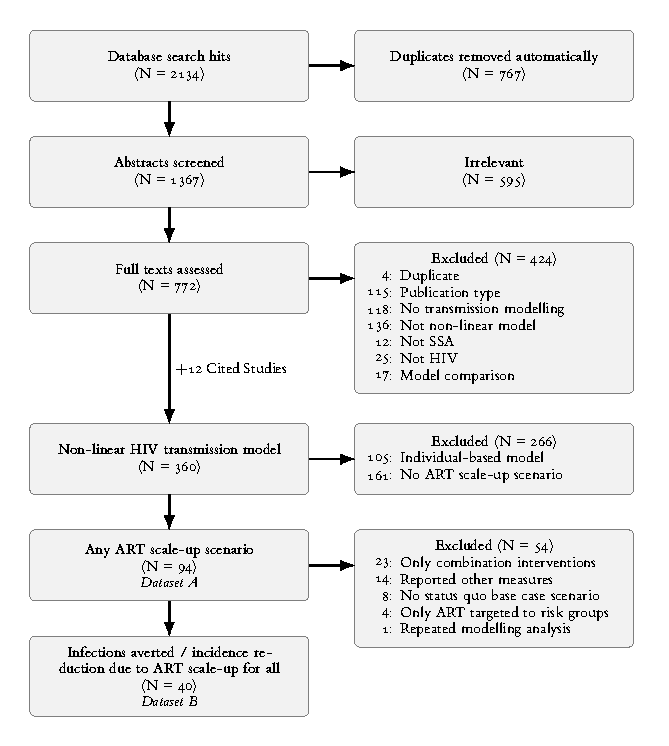
\includegraphics[width=0.8\textwidth]{prisma}
  \caption{PRISMA flowchart of study identification}
  \label{fig:prisma}
\end{figure}
% ==============================================================================
\subsection{Epidemic Context}
\label{ss:res:context}
Table~\ref{tab:summary} summarizes key features of contexts within SSA
where the prevention impacts of ART have been modelled.
\x{geo/n.any.nat} studies modelled HIV transmission at the national level;
studies also explored
regional (\x{geo/n.any.sub.ssa}),
sub-national (\x{geo/n.any.sub.nat}), and
city-level (\x{geo/n.any.city}) epidemic scales.
South Africa was the most common country simulated (\x{co/n.South-Africa} studies);
Figure~\ref{fig:map} illustrates the number of studies by country.
East Africa was the most represented SSA region, being simulated in \x{co/n.re.east} studies,
followed by Southern (\x{co/n.re.south}), West (\x{co/n.re.west}), and Central Africa (\x{co/n.re.central}).
\begin{table}
  \centering
  \caption{Summary of epidemic contexts within Sub-Saharan Africa where
    the prevention impacts of ART have been modelled}
  \label{tab:summary}
  \footnotesize\singlespacing
\begin{tabular}{llr}
	\toprule
	\multicolumn{2}{l}{Study Characteristic} & Studies               \\
	\midrule
	Geographic scale & Regional              & \x{geo/n.any.sub.ssa} \\
	                 & National              & \x{geo/n.any.nat}     \\
	                 & Sub-national          & \x{geo/n.any.sub.nat} \\
	                 & City                  & \x{geo/n.any.city}    \\
	\midrule
	Modelled         & South Africa          & \x{co/n.South-Africa} \\
	countries\tn{a}  & Kenya                 & \x{co/n.Kenya}        \\
	                 & Zambia                & \x{co/n.Zambia}       \\
	                 & Other                 & \x{co/n.Other}        \\
	\midrule
	HIV prevalence   & Low ($<$1\%)          & \x{t0/n.prev.Low}     \\
	                 & Mid (1-10\%)          & \x{t0/n.prev.Mid}     \\
	                 & High ($>$10\%)        & \x{t0/n.prev.High}    \\
	                 & Unclear/Varies        & \x{t0/n.prev.NA}      \\
	\midrule
	Incidence trend  & Decreasing            & \x{t0/n.phase.decr}   \\
	at scenario      & Dec-to-stable         & \x{t0/n.phase.dts}    \\
	divergence       & Stable                & \x{t0/n.phase.stab}   \\
	                 & Inc-to-stable         & \x{t0/n.phase.its}    \\
	                 & Increasing            & \x{t0/n.phase.incr}   \\
	                 & Unclear/Varies        & \x{t0/n.phase.NA}     \\
	\midrule
	Key populations  & FSW\tn{b}             & \x{kp/n.FSW}          \\
	included         & Clients\tn{c}         & \x{kp/n.Cli}          \\
	                 & MSM                   & \x{kp/n.MSM}          \\
	                 & PWID                  & \x{kp/n.PWID}         \\
%	                 & AGYW                  & TODO                  \\
	\bottomrule
\end{tabular}
\floatfoot{
  Total studies: \na.
  FSW: female sex workers;
  Clients: clients of sex workers;
  MSM: men who have sex with men;
  PWID: people who inject drugs;
%  AGYW: adolescent girls and young women;
%  MP: mobile populations.
  \tnt[a]{Does not sum to \na as some studies modelled multiple countries}.
  \tnt[b]{FSW as defined by three epidemiological criteria in Appendix~\ref{aaa:defs:kp};
    \x{kp/n.FSW.n.crit.3} met all three FSW criteria while
    \x{kp/n.FSW.n.crit.NA} were described as FSW but the criteria could not be evaluated;
    another \x{kp/n.FSW.n.crit.fail} were described as FSW but did not meet the criteria.}
  \tnt[c]{Likewise for clients, the counts were:
    \x{kp/n.Cli.n.crit.1},~\x{kp/n.Cli.n.crit.NA},~and~\x{kp/n.Cli.n.crit.fail}, respectively.}
}

\end{table}
\par
ART prevention impacts were most often modelled in
high-prevalence ({$>$10\%}) epidemics (\x{t0/n.prev.High} studies) and
medium-prevalence ({1-10\%}) epidemics (\x{t0/n.prev.Mid}) (Figure~\ref{fig:api.prev}).
No studies reported overall HIV prevalence of {$<$1\%} at time of intervention,
although for \x{t0/n.prev.NA} studies, HIV prevalence was
not reported or varied across simulated contexts/scenarios.
The \xdmdef year of intervention was \xdm[ ]{t0/t0}; at which time
HIV prevalence (\%) was \xdm{t0/prev} (Figure~\ref{fig:api.prev}); and
incidence (per 1000 person-years) was \xdm{t0/inc} (Figure~\ref{fig:api.inc}).
Most reported incidence trends were decreasing or stable
(45 of 48 reporting, Figure~\ref{fig:api.phase}). % MAN \x{t0/n.phase.*}
% ------------------------------------------------------------------------------
\subsubsection{Key Populations}
\label{sss:res:kp}
Groups representing FSW were described in \x{kp/n.FSW.named} studies.
Among these (of studies where it was possible to evaluate):
\x{kp/n.FSW.n.crit.p} (of \x{kp/n.FSW.n.crit.p.v}) were {$<$5\%} of the female population;
\x{kp/n.FSW.n.crit.pr} (of \x{kp/n.FSW.n.crit.pr.v}) were {$<$1/3} the size of the client population; and
\x{kp/n.FSW.n.crit.cr} (of \x{kp/n.FSW.n.crit.cr.v}) had {$>$50$\times$} partners per year versus
the lowest sexually active female activity group.
Clients of FSW were modelled as a unique group in \x{kp/n.Cli.named} studies,
among which \x{kp/n.Cli.n.crit} (of \x{kp/n.Cli.n.crit.v} reporting)
were {$>$3$\times$} the size of the FSW population.
In another \x{kp/n.Cli.named.p} studies, clients were defined as a proportion of another group,
among which \x{kp/n.Cli.n.p.crit} (of \x{kp/n.Cli.n.p.crit.v})
were {$>$3$\times$} the FSW population size.
Activity groups representing
men who have sex with men (MSM) were noted in \x{kp/n.MSM} studies;
transgender in \x{kp/n.TG};
people who inject drugs (PWID) in \x{kp/n.PWID}; and
prisoners in \x{kp/n.pris}.
% ==============================================================================
\subsection{Heterogeneity Factors}
\label{ss:res:factors}
% ------------------------------------------------------------------------------
\subsubsection{Biological Effects}
\label{sss:res:bio}
The \xdmdef number of states used to represent HIV disease
(ignoring treatment-related stratifications) was \xdm{hiv/hiv.n} (Figure~\ref{fig:hiv.n}),
and \x{hiv/n.hiv.cts} studies represented HIV along a continuous dimension
using partial differential equations.
States of increased infectiousness associated with acute infection and late-stage disease
were simulated in \x{hiv/n.hiv.acute} and \x{hiv/n.hiv.late} studies, respectively.
\par
The relative risk of HIV transmission on ART was \xdm{art/rbeta}
(Figure~\ref{fig:art.rbeta}),
representing an average ``on-treatment'' state in \x{art/n.rbeta.x.T} studies,
versus a ``virally suppressed'' state in \x{art/n.rbeta.x.V}.
Treatment failure due to drug resistance was simulated in \x{art/n.art.fail.any} studies, including:
\x{art/n.art.x.fail} where individuals experiencing treatment failure
were tracked separately from ART-naive; and
\x{art/n.art.r.fail} where such individuals
transitioned back to a generic ``off-treatment'' state.
Another \x{art/n.art.r.frop} studies included a similar transition
that was not identified as treatment failure versus ART cessation.
Transmissible drug resistance was simulated in \x{art/n.tdr} studies.
% ------------------------------------------------------------------------------
\subsubsection{Behavioural Effects}
\label{sss:res:beh}
Reduced sexual activity during late-stage HIV was simulated in \x{hiv/n.hiv.morb.any} studies,
including at least one state with:
complete cessastion of sexual activity (\x{hiv/n.hiv.morb.inact});
reduced rate/number of partnerships (\x{hiv/n.hiv.morb.np}); and/or
reduced rate/number of sex acts per partnership (\x{hiv/n.hiv.morb.vol}).
\par
Separate health states representing diagnosed HIV before treatment,
and on-treatment before viral suppression were simulated in
\x{art/n.art.x.dx} and \x{art/n.art.x.vlus} studies, respectively.
\x{art/n.bc.any} studies modelled behaviour changes following awareness of HIV+ status, including:
increased condom use (\x{art/n.bc.cond.any});
fewer partners per year (\x{art/n.dx.bc.np});
fewer sex acts per partnership (\x{art/n.dx.bc.vol});
serosorting (\x{art/n.dx.bc.ss}); and/or
a generic reduction in transmission probability (\x{art/n.dx.bc.gen}).
\par
ART cessation was simulated in \x{art/n.art.drop.any} studies, including:
\x{art/n.art.x.drop} where individuals no longer on ART
were tracked separately from ART-naive; and
\x{art/n.art.r.drop} where such individuals
transitioned back to a generic ``off-treatment'' state.
Another \x{art/n.art.r.frop} studies included a similar transition
that was not identified as treatment failure versus ART cessation.
% ------------------------------------------------------------------------------
\subsubsection{Network Effects}
\label{sss:res:network}
Populations were stratified by activity (different rates and/or types of partnerships formed)
in \x{act/n.act.def.np} studies, and by sex/gender in \x{act/n.act.def.sex}.
The number of groups defined by sex/gender and/or activity was \xdm{act/act.n}  (Figure~\ref{fig:act.n});
and by activity alone (maximum number of groups among:
women who have sex with men, men who have sex with women,
MSM, or overall if sex/gender was not considered) was \xdm{act/act.n.z}.
The highest activity groups for females and males (possibly including FSW/clients) comprised
\xdm{act/hrw.p} and \xdm{act/hrm.p}\% of female and male populations, respectively
(Figures~\ref{fig:act.HRW.p}~and~\ref{fig:act.HRM.p}).
\par
Turnover between activity groups and/or key populations
was considered in \x{act/n.turnover.any} studies,
of which \x{act/n.turnover.high} considered turnover of only
one specific high-activity group or key population.
Another \x{act/n.turnover.repl} studies simulated
movement only from lower to higher activity groups
to re-balance group sizes against disproportionate HIV mortality.
\par
Among \x{act/n.act.def.np} studies with activity groups, sexual mixing was modelled as
assortative in \x{pt/n.mix.asso} and proportionate in \x{pt/n.mix.prop}.
Partnerships had equal probability of transmission in \x{pt/n.pt.gen} studies,
including all studies without activity groups.
Partnerships were defined by the activity groups involved in \x{pt/n.pt.grp} studies,
among which transmission was usually
lower in high-with-high activity partnerships than in low-with-low, due to
fewer sex acts (\x{pt/n.grp.vol}) and/or increased condom use (\x{pt/n.grp.condom}).
Transmission risk in high-with-low activity partnerships was defined by the:
susceptible partner (\x{pt/n.act.drive.sus});
lower activity partner (\x{pt/n.act.drive.low});
higher activity partner (\x{pt/n.act.drive.high}); or
both partners' activity groups (\x{pt/n.act.drive.mix});
yielding indeterminate, higher, lower, or intermediate
per-partnership transmission risk, respectively.
Partnerships were defined based on overlapping types, such that
different partnership types could be formed between the same two activity groups in \x{pt/n.pt.phen} studies.
All overlapping partnership types had differential total sex acts and condom use.
\par
Age groups were simulated in \x{age/n.age.any} studies, among which,
the number of age groups was \xdm{age/age.n} (Figure~\ref{fig:age.n}),
and \x{age/n.age.cts} studies simulated age along a continuous dimension.
Sexual mixing between age groups was assumed to be assortative
either with (\x{age/n.mix.offd}) or without (\x{age/n.mix.asso})
average age differences between men and women;
or proportionate (\x{age/n.mix.prop}).
Differential risk behaviour by age was modelled in \x{age/n.risk} studies.
% ------------------------------------------------------------------------------
\subsubsection{Coverage Effects}
\label{sss:res:cov}
Differential transition rates along the ART cascade were considered in
\x{cov/n.diff.any.any} studies, including differences between
genders in \x{cov/n.diff.any.sex};
age groups in \x{cov/n.diff.any.age}; and
key populations in \x{cov/n.diff.any.kp}.
Another \x{cov/n.diff.any.any.j} studies did not simulate differential cascade transitions,
but justified the decision using context-specific data.
Differences between genders included rates of
HIV diagnosis (\x{cov/n.diff.dx.sex});
ART initiation (\x{cov/n.diff.art.i.sex}); and
ART cessation (\x{cov/n.diff.art.o.sex}),
with cascade engagement higher among women,
in most cases attributed to antenatal services.
Differences between age groups also affected
rates of diagnosis (\x{cov/n.diff.dx.age});
ART initiation (\x{cov/n.diff.art.i.age});
but not ART cessation (\x{cov/n.diff.art.o.age}). % MAN
Among key populations, \emph{lower} rates of
diagnosis, ART initiation, and retention were simulated in
\x{cov/n.diff.dx.kp}, \x{cov/n.diff.art.i.kp}, and \x{cov/n.diff.art.o.kp}
studies respectively, while \emph{higher} rates were simulated in
\x{cov/n.diff.dx.kp.H}, \x{cov/n.diff.art.i.kp.H}, and \x{cov/n.diff.art.o.kp.H}.
% ==============================================================================
\subsection{ART Prevention Impact}
\label{ss:res:api}
Dataset~B comprised \x{n/n.a.api} studies,
including \x{n/n.s.api} scenarios of ART scale-up.
Relative incidence reduction (IR) with ART scale-up as compared to status quo
was reported in \x{n/n.a.api.inc} studies (\x{n/n.s.api.inc} scenarios);
proportion of cumulative infections averted (CIA) due to ART scale-up
was reported in \x{n/n.a.api.chi} (\x{n/n.s.api.chi});
and \x{n/n.a.api.both} (\x{n/n.s.api.both}) reported both.
Some scenarios included multiple time horizons.
\par
\begin{table}
  \centering
  \caption{Projected ART prevention impacts,
    stratified by factors of risk heterogeneity and contexts}
  \newcommand{\xtab}[1]{\x{api/inc/#1.xtab} & \x{api/chi/#1.xtab} }%
\def\baselinestretch{1.1}\footnotesize%
\centerline{%
\setlength{\tabcolsep}{.7ex}%
\begin{tabular}{ll rrc rc rrc rc}
  \toprule
  & & \multicolumn{5}{c}{Incidence Reduction (\%)}
    & \multicolumn{5}{c}{Cumulative Infections Averted (\%)} \\
  \cmidrule(rl){3-7}\cmidrule(rl){8-12}
  Factor               & Level            & N\tn{a} & Median & (IQR) & Effect\tn{b} & (95\% CI)\tn{b} 
                                          & N\tn{a} & Median & (IQR) & Effect\tn{b} & (95\% CI)\tn{b} \\
  \midrule
%%\begin{tabular}{lll}
  Time Horizon         & 0-10             & \xtab{t.cat.0}               \\
  (years)              & 11-20            & \xtab{t.cat.10}              \\
                       & 21-30            & \xtab{t.cat.20}              \\
                       & 31+              & \xtab{t.cat.30}              \\[\tsep]
  HIV Prevalence       & 10+              & \xtab{api.prev.cat.High}     \\
  (\%)                 & 1-10             & \xtab{api.prev.cat.Mid}      \\
                       & 0-1              & \xtab{api.prev.cat.Low}      \\[\tsep]
  HIV Incidence        & Increasing       & \xtab{api.phase.incr}        \\
  Trend\tn{c}          & Inc-to-stable    & \xtab{api.phase.its}         \\
                       & Stable           & \xtab{api.phase.stab}        \\
                       & Dec-to-stable    & \xtab{api.phase.dts}         \\
                       & Decreasing       & \xtab{api.phase.decr}        \\
  \midrule
  RR Transmission      & 0.0-0.039        & \xtab{art.rbeta.cat.0}       \\
  on ART               & 0.04-0.099       & \xtab{art.rbeta.cat.0.04}    \\
                       & 0.1+             & \xtab{art.rbeta.cat.0.1}     \\[\tsep]
  CD4 Threshold for    & Symptomatic      & \xtab{art.cd4.symp}          \\
  ART Initiation       & 200              & \xtab{art.cd4.200}           \\
                       & 350              & \xtab{art.cd4.350}           \\
                       & 500              & \xtab{art.cd4.500}           \\
                       & Any              & \xtab{art.cd4.All}           \\
                       & Mixed            & \xtab{art.cd4.*}             \\[\tsep]
  ART Coverage         & 0-59             & \xtab{art.cov.cat.0}         \\
  Target (\%)\tn{c}    & 60-84            & \xtab{art.cov.cat.0.6}       \\
                       & 85+              & \xtab{art.cov.cat.0.85}      \\
  \midrule
  Acute Infection      & No               & \xtab{hiv.x.acute.FALSE}     \\
                       & Yes              & \xtab{hiv.x.acute.TRUE}      \\[\tsep]
  Late-Stage Infection & No               & \xtab{hiv.x.late.FALSE}      \\
                       & Yes              & \xtab{hiv.x.late.TRUE}       \\[\tsep]
  Trans. Drug Resist.  & No               & \xtab{art.tdr.FALSE}         \\
                       & Yes              & \xtab{art.tdr.TRUE}          \\
  \midrule
  HIV Morbidity        & No               & \xtab{hiv.morb.any.FALSE}    \\
                       & Any              & \xtab{hiv.morb.any.TRUE}     \\[\tsep]
  HTC Behav. Change    & No               & \xtab{bc.any.FALSE}          \\
                       & Any              & \xtab{bc.any.TRUE}           \\
  \midrule
  Risk Definition      & None             & \xtab{Risk.None}             \\
                       & Activity (No KP) & \xtab{Risk.Activity-(no-KP)} \\
                       & KP (Priority)    & \xtab{Risk.KP-(priority)}    \\
                       & KP (Same)        & \xtab{Risk.KP-(same)}        \\[\tsep]
  Activity Turnover    & No               & \xtab{act.turn.any.FALSE}    \\
                       & Yes              & \xtab{act.turn.any.TRUE}     \\[\tsep]
  Partnership Types    & Generic          & \xtab{pt.def.gen}            \\
                       & By Groups        & \xtab{pt.def.grp}            \\
                       & Overlapping      & \xtab{pt.def.phen}           \\[\tsep]
  Sex Stratification   & No               & \xtab{act.def.sex.FALSE}     \\
                       & Yes              & \xtab{act.def.sex.TRUE}      \\
  \bottomrule
\end{tabular}}
\floatfoot{
  \tnt[a]{N: number of unique scenarios and time horizons;
    sums across factor levels may be less than 126 and 115 due to missing variables.}
  \tnt[b]{Effect estimates from linear multivariate regression
    with generalized estimating equations \cite{Hojsgaard2006};
    effects are illustrated in Figure~\ref{fig:effects}.}
  \tnt[c]{Omitted from regression model due to missing data.}
  RR: relative risk;
  HTC: HIV testing and counselling;
  KP: key populations.
  priority: modelled ART cascade transitions were faster in KP vs overall due to prioritized programs;
  same: cascade transitions were assumed the same in KP as overall.
  Factor definitions are given in Appendix~\ref{a:defs}.
}

  \label{tab:api}
\end{table}
\begin{figure}
  \centering
  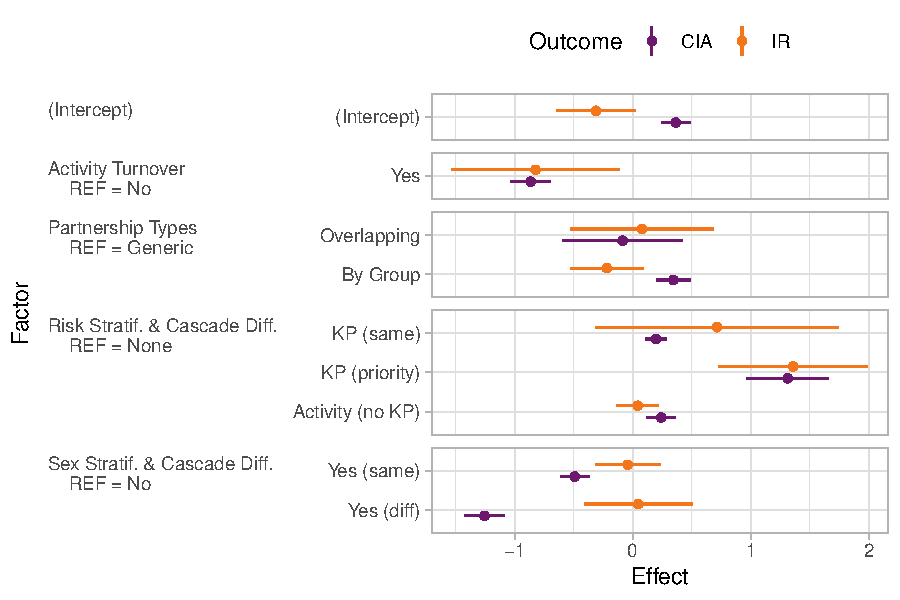
\includegraphics[width=0.75\linewidth]{effects-subset}
  \caption{Effect estimates for selected factors of heterogeneity on
    incidence reduction (\%, IR) and cumulative infections averted (\%, CHI)
    from linear multivariate regression with generalized estimating equations.}
  \label{fig:effects-sub}
  \floatfoot{
    Numerical results given in Table~\ref{tab:api}.
    KP: key populations.
    priority: modelled ART cascade transitions were faster in KP vs overall due to prioritized programs;
    same: cascade transitions were assumed the same in KP as overall;
    diff: cascade transitions were slower among men.
    Factor definitions are given in Appendix~\ref{a:defs}.}
\end{figure}
Table~\ref{tab:api} summarizes projected ART prevention impacts (IR, CIA),
stratified by heterogeneity and contextual factors,
plus adjusted effect estimates for each factor from multivariate analysis.
Figures~\ref{fig:api:Risk}--\ref{fig:api:art.rbeta.cat} illustrate
unadjusted impacts stratified by factor levels, while
Figures~\ref{fig:effects}~and~\ref{fig:effects-sub} (subset) illustrate effect estimates.
Including activity groups without key populations
slightly increased projected ART prevention impacts---adjusted effect (95\% CI):
\x{api/inc/Risk.Activity-(no-KP).eff}\% IR, \x{api/chi/Risk.Activity-(no-KP).eff}\% CIA.
Including key population(s) without prioritized ART cascade had a similar effect:
\x{api/inc/Risk.KP-(same).eff}\% IR, \x{api/chi/Risk.KP-(same).eff}\% CIA.
However, including turnover of one or more higher risk group(s) reduced ART prevention impacts:
\x{api/inc/act.turn.any.TRUE.eff}\% IR, \x{api/chi/act.turn.any.TRUE.eff}\% CIA,
such that overall, including activity groups and/or key population(s) with turnover
reduced ART prevention impacts.
\par
Including ART cascade prioritized to any key population(s)
increased the projected ART prevention impacts enough to overcome reductions due to turnover:
\x{api/inc/Risk.KP-(priority).eff}\% IR, \x{api/chi/Risk.KP-(priority).eff}\% CIA.
No studies in Dataset~B examined lower ART cascade among key population(s).
Stratifying by sex/gender, and considering lower ART cascade among men was estimated to reduce CIA:
\x{api/chi/Sex.Yes-(same).eff}\% and \x{api/chi/Sex.Yes-(diff).eff}\%, respectively;
although similar effects were not observed for IR:
\x{api/inc/Sex.Yes-(same).eff}\% and \x{api/inc/Sex.Yes-(diff).eff}\%.